
%%
%% Conference Paper for IRC'20, November 9-11, Taichung, Taiwan
%% ***
%%

\documentclass[conference]{IEEEtran}
%\documentclass[conference, onecolumn, draftclsnofoot]{IEEEtran}

\newcommand{\stt}[1]{{\small\tt #1}} %\small\tt too small here
\newcommand{\powprof}{\stt{powprofiler}}
\newcommand{\figpath}{./figures}
\let\labelindent\relax

%\usepackage{lineno}
%\linenumbers
%\usepackage[left=4cm, right=7cm]{geometry}
%\setlength{\marginparwidth}{4cm}
\usepackage[inline]{enumitem}
\usepackage{booktabs}
\usepackage{flushend}
\usepackage{tikz}
\usepackage{siunitx}
\sisetup{per-mode = symbol}
\DeclareSIUnit\fps{fps}
\usepackage{todonotes}
\setuptodonotes{inline}
%\newcommand{\adam}[2][]{\todo[color=orange!20, #1]{ADAM: #2}}
%\newcommand{\hemi}[2][]{\todo[color=green!20, #1]{HEMI: #2}}


%% citation packege
\usepackage{cite}

%% figures package
\usepackage{graphicx}
\graphicspath{{figures/}}
%\DeclareGraphicsExtensions{.pdf,.jpeg,.png}

%% math package
\usepackage[cmex10]{amsmath}
\usepackage{mathtools}
\usepackage{amssymb}

%% pseudocode package
%\usepackage{algorithmic}

%% packages for alignment
%\usepackage{array}
%\usepackage{mdwmath}
%\usepackage{mdwtab}
%\usepackage{eqparbox}

%% packages for subfigures (eventually)
\usepackage[tight,footnotesize]{subfigure}
%S\usepackage[caption=false]{caption}
%\usepackage[font=footnotesize]{subfig}
%\usepackage[caption=false,font=footnotesize]{subfig}

%% package for urls
\usepackage{url}

%% correct bad hyphenation here
\hyphenation{analysis}

%% references (generates a bib file for bibtex)
\begin{filecontents}{\jobname.bib}
@article{salami2014uav,
  title={{UAV} flight experiments applied to the remote sensing of vegetated areas},
  author={Salam{\'\i}, Esther and Barrado, Cristina and Pastor, Enric},
  journal={Remote Sensing},
  volume={6},
  number={11},
  pages={11051--11081},
  year={2014},
  publisher={Multidisciplinary Digital Publishing Institute}
}
@inproceedings{costa2012use,
  title={The use of unmanned aerial vehicles and wireless sensor network in agricultural applications},
  author={Costa, Fausto G and Ueyama, J{\'o} and Braun, Torsten and Pessin, Gustavo and Os{\'o}rio, Fernando S and Vargas, Patr{\'\i}cia A},
  booktitle={2012 IEEE International Geoscience and Remote Sensing Symposium},
  pages={5045--5048},
  year={2012},
  organization={IEEE}
}
@inproceedings{seewald2020mechanical,
  title={Mechanical and Computational Energy Estimation of a Fixed-Wing Drone}, 
  author={Seewald, Adam and Garcia de Marina, Hector and Midtiby, Henrik Skov and Schultz, Ulrik Pagh},
  booktitle={2020 4th IEEE International Conference on Robotic Computing (IRC)},
  pages={to appear},
  year={2020},
  organization={IEEE} 
}
@inproceedings{saripalli2002vision,
  title={Vision-based autonomous landing of an unmanned aerial vehicle},
  author={Saripalli, Srikanth and Montgomery, James F and Sukhatme, Gaurav S},
  booktitle={2002 IEEE International Conference on Robotics and Automation (ICRA)},
  volume={3},
  pages={2799--2804},
  year={2002},
  organization={IEEE}
}

@inproceedings{saripalli2003landing,
  title={Landing on a moving target using an autonomous helicopter},
  author={Saripalli, Srikanth and Sukhatme, Gaurav S},
  booktitle={Field and Service Robotics},
  pages={277--286},
  year={2003},
  organization={Springer}
}

@inproceedings{lee2012autonomous,
  title={Autonomous landing of a {VTOL UAV} on a moving platform using image-based visual servoing},
  author={Lee, Daewon and Ryan, Tyler and Kim, H Jin},
  booktitle={2012 IEEE International Conference on Robotics and Automation (ICRA)},
  pages={971--976},
  year={2012},
  organization={IEEE}
}

@inproceedings{chen2016system,
  title={System integration of a vision-guided {UAV} for autonomous landing on moving platform},
  author={Chen, Xudong and Phang, Swee King and Shan, Mo and Chen, Ben M},
  booktitle={2016 12th IEEE International Conference on Control and Automation (ICCA)},
  pages={761--766},
  year={2016},
  organization={IEEE}
}
@inproceedings{falanga2017vision,
  title={Vision-based autonomous quadrotor landing on a moving platform},
  author={Falanga, Davide and Zanchettin, Alessio and Simovic, Alessandro and Delmerico, Jeffrey and Scaramuzza, Davide},
  booktitle={2017 IEEE International Symposium on Safety, Security and Rescue Robotics (SSRR)},
  pages={200--207},
  year={2017},
  organization={IEEE}
}	
@article{araar2017vision,
  title={Vision based autonomous landing of multirotor {UAV} on moving platform},
  author={Araar, Oualid and Aouf, Nabil and Vitanov, Ivan},
  journal={Journal of Intelligent \& Robotic Systems},
  volume={85},
  number={2},
  pages={369--384},
  year={2017},
  publisher={Springer}
}
@article{feng2018autonomous,
  title={Autonomous landing of a {UAV} on a moving platform using model predictive control},
  author={Feng, Yi and Zhang, Cong and Baek, Stanley and Rawashdeh, Samir and Mohammadi, Alireza},
  journal={Drones},
  volume={2},
  number={4},
  pages={34},
  year={2018},
  publisher={Multidisciplinary Digital Publishing Institute}
}
@article{kyristsis2016towards,
  title={Towards autonomous modular {UAV} missions: The detection, geo-location and landing paradigm},
  author={Kyristsis, Sarantis and Antonopoulos, Angelos and Chanialakis, Theofilos and Stefanakis, Emmanouel and Linardos, Christos and Tripolitsiotis, Achilles and Partsinevelos, Panagiotis},
  journal={Sensors},
  volume={16},
  number={11},
  pages={1844},
  year={2016},
  publisher={Multidisciplinary Digital Publishing Institute}
}
@inproceedings{acuna2018vision,
  title={Vision-based {UAV} landing on a moving platform in {GPS} denied environments using motion prediction},
  author={Acuna, Raul and Zhang, Ding and Willert, Volker},
  booktitle={2018 Latin American Robotic Symposium, 2018 Brazilian Symposium on Robotics (SBR) and 2018 Workshop on Robotics in Education (WRE)},
  pages={515--521},
  year={2018},
  organization={IEEE}
}
@inproceedings{lee2016vision,
  title={Vision-based {UAV} landing on the moving vehicle},
  author={Lee, Hanseob and Jung, Seokwoo and Shim, David Hyunchul},
  booktitle={2016 International Conference on Unmanned Aircraft Systems (ICUAS)},
  pages={1--7},
  year={2016},
  organization={IEEE}
}
@article{nguyen2018lightdenseyolo,
  title={{LightDenseYOLO}: A fast and accurate marker tracker for autonomous {UAV} landing by visible light camera sensor on drone},
  author={Nguyen, Phong Ha and Arsalan, Muhammad and Koo, Ja Hyung and Naqvi, Rizwan Ali and Truong, Noi Quang and Park, Kang Ryoung},
  journal={Sensors},
  volume={18},
  number={6},
  pages={1703},
  year={2018},
  publisher={Multidisciplinary Digital Publishing Institute}
}
@article{guo2020precision,
  title={Precision Landing Test and Simulation of the Agricultural {UAV} on Apron},
  author={Guo, Yangyang and Guo, Jiaqian and Liu, Chang and Xiong, Hongting and Chai, Lilong and He, Dongjian},
  journal={Sensors},
  volume={20},
  number={12},
  pages={3369},
  year={2020},
  publisher={Multidisciplinary Digital Publishing Institute}
}
@article{yuan2018hierarchical,
  title={A hierarchical vision-based localization of rotor unmanned aerial vehicles for autonomous landing},
  author={Yuan, Haiwen and Xiao, Changshi and Xiu, Supu and Zhan, Wenqiang and Ye, Zhenyi and Zhang, Fan and Zhou, Chunhui and Wen, Yuanqiao and Li, Qiliang},
  journal={International Journal of Distributed Sensor Networks},
  volume={14},
  number={9},
  year={2018},
  publisher={SAGE Publications Sage UK: London, England}
}
@article{yang2018hybrid,
  title={Hybrid camera array-based {UAV} auto-landing on moving {UGV} in {GPS}-denied environment},
  author={Yang, Tao and Ren, Qiang and Zhang, Fangbing and Xie, Bolin and Ren, Hailei and Li, Jing and Zhang, Yanning},
  journal={Remote Sensing},
  volume={10},
  number={11},
  pages={1829},
  year={2018},
  publisher={Multidisciplinary Digital Publishing Institute}
}
@inproceedings{olson2011apriltag,
  title={{AprilTag:} A robust and flexible visual fiducial system},
  author={Olson, Edwin},
  booktitle={2011 IEEE International Conference on Robotics and Automation (ICRA)},
  pages={3400--3407},
  year={2011},
  organization={IEEE}
}
@article{berenz2012autonomous,
  title={Autonomous battery management for mobile robots based on risk and gain assessment},
  author={Berenz, Vincent and Tanaka, Fumihide and Suzuki, Kenji},
  journal={Artificial Intelligence Review},
  volume={37},
  number={3},
  pages={217--237},
  year={2012},
  publisher={Springer}
}
@inproceedings{mei2005case,
  title={A case study of mobile robot's energy consumption and conservation techniques},
  author={Mei, Yongguo and Lu, Yung-Hsiang and Hu, Y Charlie and Lee, CS George},
  booktitle={2005 12th International Conference on Advanced Robotics (ICRA)},
  pages={492--497},
  year={2005},
  organization={IEEE}
}
@inproceedings{mei2004energy,
  title={Energy-efficient motion planning for mobile robots},
  author={Mei, Yongguo and Lu, Yung-Hsiang and Hu, Y Charlie and Lee, CS George},
  booktitle={2004 IEEE International Conference on Robotics and Automation (ICRA)},
  volume={5},
  pages={4344--4349},
  year={2004},
  organization={IEEE}
}
@article{mei2006deployment,
  title={Deployment of mobile robots with energy and timing constraints},
  author={Mei, Yongguo and Lu, Yung-Hsiang and Hu, Yu Charlie and Lee, CS George},
  journal={IEEE Transactions on Robotics},
  volume={22},
  number={3},
  pages={507--522},
  year={2006},
  publisher={IEEE}
}
@article{morales2009power,
  title={Power consumption modeling of skid-steer tracked mobile robots on rigid terrain},
  author={Morales, Jesus and Martinez, Jorge L and Mandow, Anthony and Garc{\'\i}a-Cerezo, Alfonso J and Pedraza, Salvador},
  journal={IEEE Transactions on Robotics},
  volume={25},
  number={5},
  pages={1098--1108},
  year={2009},
  publisher={IEEE}
}
@article{seewald2019coarse,
  title={Coarse-Grained Computation-Oriented Energy Modeling for Heterogeneous Parallel Embedded Systems},
  author={Seewald, Adam and Schultz, Ulrik Pagh and Ebeid, Emad and Midtiby, Henrik Skov},
  journal={International Journal of Parallel Programming},
  pages={1--22},
  year={2019},
  publisher={Springer}
}
@inproceedings{nardi2015introducing,
  title={Introducing {SLAMBench}, a performance and accuracy benchmarking methodology for SLAM},
  author={Nardi, Luigi and Bodin, Bruno and Zia, M Zeeshan and Mawer, John and Nisbet, Andy and Kelly, Paul HJ and Davison, Andrew J and Luj{\'a}n, Mikel and O'Boyle, Michael FP and Riley, Graham and others},
  booktitle={2015 IEEE International Conference on Robotics and Automation (ICRA)},
  pages={5783--5790},
  year={2015},
  organization={IEEE}
}
@article{sadrpour2013mission,
  title={Mission Energy Prediction for Unmanned Ground Vehicles Using Real-time Measurements and Prior Knowledge},
  author={Sadrpour, Amir and Jin, Jionghua and Ulsoy, A Galip},
  journal={Journal of Field Robotics},
  volume={30},
  number={3},
  pages={399--414},
  year={2013},
  publisher={Wiley Online Library}
}
@inproceedings{sadrpour2013experimental,
  title={Experimental validation of mission energy prediction model for unmanned ground vehicles},
  author={Sadrpour, Amir and Jin, Judy and Ulsoy, A Galip},
  booktitle={2013 American Control Conference},
  pages={5960--5965},
  year={2013},
  organization={IEEE}
}

@misc{NfoldMarker,
    title = "{N-fold marker tracker repository}",
    author="{Henrik Skov Midtiby}",
    year = "2015",
    howpublished = "\url{https://github.com/henrikmidtiby/MarkerLocator}"
}

@misc{ArUco_marker,
    title = "{Detection of {ArUco} markers}",
    author="{OpenCV}",
    year = "2020",
    howpublished = "\url{https://docs.opencv.org/3.4/d5/dae/tutorial_aruco_detection.html}"
}

@misc{Dynamic_pressure_NASA,
    title = "{Dynamic pressure {(NASA)}}",
    author="{NASA}",
    year = "2020",
    howpublished = "\url{https://www.grc.nasa.gov/WWW/K-12/airplane/dynpress.html}"
}

@book{anderson2010fundamentals,
  title={Fundamentals of aerodynamics},
  author={Anderson Jr, John David},
  year={2010},
  publisher={Tata McGraw-Hill Education}
}

@article{yolov3,
  title={{YOLOv3}: An Incremental Improvement},
  author={Redmon, Joseph and Farhadi, Ali},
  journal = {arXiv},
  year={2018}
}

@misc{bjelonicYolo2018,
  author = {Marko Bjelonic},
  title = {{YOLO ROS}: Real-Time Object Detection for {ROS}},
  howpublished = {\url{https://github.com/leggedrobotics/darknet_ros}},
  year = {2016--2018},
}

\end{filecontents}

\begin{document}

%% [Ad: typo] ...quadrocopter... -> ...quadcopter... {I would actually use multirotor UAV / not only quadrotors}
%% [Ad: little suggestion] An Energy-Efficient Vision-Based Autonomous Tracking and Landing Approach for a Multirotor UAV on a Moving Platform in an Agricultural Use-Case


% [Ad: Quadrocopter; so it should work as well despite what I said earlier, but I checked IEEExplore and Quadrotor is far more used]
%\title{Energy-Sensitive Vision-Based Autonomous Tracking and Landing of a Multirotor on a Moving Platform} 
\title{Energy-Sensitive Vision-Based Autonomous\\Tracking and Landing of a UAV} 
%\title{Vision-Based Autonomous Tracking and Landing of a Multirotor on a Moving Platform} 
%for an Agricultural Application %UPS: suggested title, agriculture less important, playing with "energy sensitive" since we know about the energy and can adapt QoS accordingly
%UPS: suggesting multirotor, we don't care how many rotors it has...
%\title{Energy-Sensitive Vision-Based Autonomous Tracking and Landing of a Quadrocopter on a Moving Platform} %for an Agricultural Application %UPS: suggested title, agriculture less important, playing with "energy sensitive" since we know about the energy and can adapt QoS accordingly

%% author names and affiliations
\author{
\IEEEauthorblockN{Georgios Zamanakos, Adam Seewald, Henrik Skov Midtiby, and Ulrik Pagh Schultz}
\IEEEauthorblockA{SDU UAS Center, M{\ae}rsk Mc-Kinney M{\o}ller Institute, University of Southern Denmark\\
Contact email: ups@mmmi.sdu.dk
}}

%% make the title area
\maketitle


\begin{abstract}

%\boldmath
In this paper, we present a robust, vision-based %Ulrik: downplaying the energy-sensitive thingie slightly
algorithm for autonomous tracking and landing on a moving platform 
in varying environmental conditions. We use
a novel landing marker robust to occlusions to track the moving
platform and the YOLOv3-tiny CNN to detect ground-based hazards in an agricultural use case. We
perform all computations onboard using an NVIDIA Jetson Nano and analyse %we attempt to 
% X [Ad3:]\emph in the abstract? Eventually put it back (it was \emph{NVIDIA Jetson Nano})
the impact on the flight time by profiling the energy consumption of the
landing marker detection algorithm and YOLOv3-tiny CNN. %We conduct
Experiments are conducted in Gazebo simulation using an energy
% X [Ad3:] then it's not consistent with formatting (used modeling tool instead of powp\emph{powprofiler}rofiler)
modeling tool to measure the energy cost as a function of QoS. %for autonomous
% X [Ad3:] acronym shouldn't be explained in the abstract but at first occurrence in the paper (I mean you can do it but then I'd expect the same for CNN and UAV)
%tracking and landing. 
Our experiments test the energy efficiency and
robustness of our system in various dynamic wind
disturbances. %Furthermore it is 
We show that the landing marker
detection algorithm can be run at the highest QoS with only a marginal
energy overhead whereas adapting the QoS level of YOLOv3-tiny CNN
results in a considerable power saving for the system as a whole. The
power saving is significant for a system executing on a
fixed-wing UAV but only marginal if executing on a standard multirotor UAV.

% X [Ad2:] Typo: In this paper, [grammarly does this...]
% X [Ad2:] Typo: onboard
% X [Ad2:] Typo: fixed-wing
% X [Ad2:] Since the reader has no idea what powprofiler is at this point, I suggest using 'an energy modeling tool' instead.
% X [Ad2:] Quality of Service (QoS) why to explain the acronym; I suppose it should be just QoS while it's properly introduced at first occurrence in the Introduction
% X [Ad2:] Various dynamic wind disturbances sounds confusing; I guess we might use dynamic only.


\end{abstract}

% For peer review papers, you can put extra information on the cover
% page as needed:
% \ifCLASSOPTIONpeerreview
% \begin{center} \bfseries EDICS Category: 3-BBND \end{center}
% \fi
%
% For peerreview papers, this IEEEtran command inserts a page break and
% creates the second title. It will be ignored for other modes.
\IEEEpeerreviewmaketitle



%%%%%%%%%%%%%%%%%%%%%%
\section{Introduction}
\label{sec:introduction}

Unmanned Aerial Vehicles (UAVs) are increasingly used for applications
such as monitoring, surveillance, transportation of small payloads,
and agricultural applications~\cite{costa2012use,salami2014uav}.
%
One of the major constraints of such applications is their limited level of autonomy due to battery limitations. %It is therefore seen that to further 
%
Extending the flying time of a UAV is normally done by having it land
in order to replace or charge the battery before continuing the
mission. Performing landings autonomously can however be challenging
depending on the environment and whether the landing platform is
stationary or mobile.
%
%Apart from presenting an increased energy efficiency concerning the computations, our approach further elaborates on the landing of the UAV on a moving platform. It can be easily shown that it is not generally energy- or time-efficient for the UAV to fly back to its base, once the battery reaches a critical level. Instead it is proposed that the UAV should land on the moving vehicle that is inherently in the proximity of the UAV during normal operation. 
%
Moreover, relying solely on the availability of a GPS signal for
autonomous precision landing is not considered safe, since GPS signals
can be temporarily lost or even tampered with.
%
%The noise and errors of the GPS signal are not predictable and instead a 
%
As an alternative, in this paper we investigate the use of a novel
vision-based autonomous landing system and evaluate its robustness
towards environmental conditions such as visual disturbances and wind.
%
%is considered a more optimal option.

% X [Ad2:] Typo: in this paper, X [Ad3:] oko this doesn't sound that good after the comma anyways
% X [Ad2:] Typo: landing system and

Extension of the flight time can be also achieved by using
\emph{energy-sensitive algorithms} that can reduce energy consumption
by reducing the Quality of Service (QoS). With this approach,
energy-costly computations such as computer vision are adapted by
selecting the desired quality of service to match the available
energy~\cite{seewald2020mechanical}.
%
%With such an approach,
%
By combining energy-sensitive algorithms with autonomous landing
capabilities, we aim to increase the total availability of the UAV to
perform operations, by extending the flight time and using autonomous
recharging when needed.
%
%reduce the energy consumption of the UAV during flight and furthermore increase the level of autonomy.

% X [Ad2:] Quality of Service (QoS)

The main contribution of this paper concerns the experimental study of
a robust vision-based algorithm for autonomous
tracking and landing in varying environmental conditions. The
algorithms are executed on an NVIDIA Jetson Nano companion computer
controlling a simulated drone. The vision-based tracking and landing
algorithms provide novel capabilities in terms of tolerance to visual
disturbance and varying environmental conditions such as wind.
%
Our experiments are based on an agricultural use-case where a
multirotor UAV performs visual identification of ground-based hazards
while tracking and landing on a moving platform.
%
%will be studied.

% X [Ad2:] NVIDIA here but Nvidia in abstract {I guess it should be NVIDIA}



%%%%%%%%%%%%%%%%%%%%%%
\section{State of the Art}
\label{sec:state-of-the-art}

Vision-based autonomous landing on a marker has been extensively
studied by many researchers. Key distinctions include whether the
marker is on a moving platform, the type of the marker, the algorithms
used to detect it, as well as the mounted sensors onboard of the UAV.

For stationary platforms, one of the first experiments with
vision-based autonomous landing was conducted by Saripalli
et~al.~\cite{saripalli2002vision}. Here, a helicopter with a color
camera facing vertically towards the ground would land on an ”H”-shape
pattern (similar to ones found on a helipad) using a hierarchical
behavior-based control architecture. In physical tests a marker of
\SI{122}{}$\times$\SI{122}{\cm} size was detected for a maximum altitude of \SI{10}{\m}. A
% [Ad3:] why cms twice?
landing marker inspired by a QR code but consisting of three
artificial markers is investigated by Yuan
et~al.~\cite{yuan2018hierarchical}, and was shown to provide a \SI{6}-Degree Of Freedom (DOF)
pose over an altitude range of \SI{0}{}-\SI{20}{\m}. Our work is in contrast focused on
the ability to land on moving platforms.

Saripalli et~al.~\cite{saripalli2003landing} also demonstrated the use
of a Kalman Filter to track a moving platform. However, all the
computations were performed offline. Similarly, an ArUco marker was
used as a landing marker by Lee et~al.~\cite{lee2012autonomous} to
detect a moving platform. The control of the UAV is performed based on
the error provided by the vision algorithm but all the computations
were performed off-board. Arrar et~al.~\cite{araar2017vision} focus
on extending the detection range by using an
AprilTag~\cite{olson2011apriltag} as a landing marker. Again all the
computer vision algorithms were also executed off-board. Conversely, a crucial
aspect of our application is to perform all the computations onboard,
and to evaluate them according to their energy efficiency as a
function of QoS.

% X [Ad2:] Saripalli demonstrated sounds almost like he did some formal demonstration of math-like kind of the Kalman filter variation he used. What about just used?
% X [Ad2:] I don't like that the paragraph is not self contained; it adds some information to Saripalli but goes directly to Lee. What about moving Saripalli...offline to the above paragraph?

% [Georgios2:]Saripalli and Lee both performed offline/offboard computations and that is the purpose of this paragraph. To show the importance of performing the computations onboard.

% X [Ad3:] Good, it's another Saripalli's work; thought the previous chapter was the same work (hence the confusion). Maybe later instead of also? Flows sort of better.

% X [Ad2:] Typo: if you don't stick with the above suggestion, there is a comma after However missing
% X [Ad2:] Typo: onboard

%\hemi{I think the last sentence mixes what others
%  have done and what we want to do in the paper.}

The design of the marker and choice of sensors can facilitate doing the computations onboard. %Is this the point of this paragraph?
%
Chen et~al.~\cite{chen2016system} utilized a marker consisting of a
circle and rectangles of different colors along with a LiDAR scanning
range finder for height estimation. The marker was detected by
performing color segmentation on the incoming image frame. By fusing
the height measurement from the LiDAR into the vision measurement, a
relative pose of the UAV from the moving platform was obtained. A
color segmentation approach was also implemented by Lee
et~al.~\cite{lee2016vision}. A red rectangle was used as a landing marker while the detection was done by a vertically facing camera with a fish-eye lens. The setup accounted for a successful landing from an altitude of \SI{70}{\m}. In the above two cases an onboard companion computer is used to
perform all the computations on the UAV. However, we in this work do not consider a color segmentation
approach, since for a realistic (outdoor)
case it would be difficult to ensure that the
landing marker will be the only object of a specific color in the
scene.

% X [Ad2:] Typo onboard
% X [Ad2:] it sounds little disconnected. I would do this: The design...utilized -> The design of the marker and choice of sensors can potentially facilitate the onboard computations, as investigated by Chen et~al.~\cite{chen2016system}. The approach utilized
% X [Ad2:] Sounds like the sentence "By fusing the height measurement from the LiDAR into the vision measurement, a relative pose of the UAV from the moving platform was obtained." sounds unnecessarily complicated {in fact I don't understand} -> "The relative pose of the UAV with respect to the moving platform was obtained fusing the height taken visually and using a LiDAR." {although again not sure how the height is obtained visually; seems I am missing some points so in case ignore}
% [Georgios2:] The height is not ontained visually but only from the LiDAR sensor. The vision measurement is in pixels. By combining the pixel measurement and the distance from the LiDAR we are able to find the 3d position of the target. If we do not have the distance measurement (from the LiDAR) we can only have the homogeneous coordinates of the target, not the 3d world coordinates. I would leave this sentence as it is.

% X [Ad3:] perhaps vision measurement -> distance measurement? Is vision measurement a conventional way of saying the value of the distance taken from the lidar? IDN

%[Georgios3:] I would stick to distance measurement since I think that LiDARs are not considered as vision sensors like cameras are.

% X [Ad2:] Too many times 'was used' and a little intricated; perhaps "A red rectangle was used as a landing marker and a vertically facing camera with a fish-eye lens was used to detect it, and a successful landing from an altitude of \SI{70}{\m} was demonstrated." -> "A red rectangle was used as a landing marker while the detection was done by a vertically facing camera with a fish-eye lens. The setup accounted for a successful landing from an altitude of \SI{70}{\m}."
% [Georgios2:] I like that better too. Will change it accordingly.

% X [Ad2:] teams -> approaches {teams sounds like they participated in these competitions...}
% [Georgios2:] Will add "researchers" instead of "teams"

% X [Ad3:] LOL sorry for being annoying but it's et. al. in both cases so it's not entirely clear which researchers from the et. al. :P

%[Georgios3:] No worries :P ... I rephrazed it.

% X [Ad2:] Typo: computations
% X [Ad2:] the last sentence, However...scene., is unclear. Perhaps: We do not consider a color segmentation approach due to the high variability of the outdoor environment. {actually this doesn't seem entirely correct; maybe we could omit. I mean, if they landed from 70 meters they probably weren't in a lab with a white background and a colored marker in the middle...}

%[Georgios2:] We do not know the environment that they performed the landing. Although outside, a red car present in the scene might cause their algorithm to fail. I would suggest keeping that as it is.

% X [Ad3:] yes, but it sounds we are criticizing them while we are not even stating in that sentence what we are using instead (if I am a reviewer and I see somebody taking such position I start questioning). I would be rather conservative. Maybe omitting However on?

%[Georgios3:] I would consider as an assumption we make to increase the overall robustness. I am ok in omitting it if it seems too criticizing

% [Ad4:] Good; I see the point, the reader might not though. Rephrased a little to be more 'gentle' (without as a safe option, and if not impossible)

The use of a hybrid camera system consisting of a fish-eye IR camera
and a stereo camera was demonstrated by Yang
et~al.~\cite{yang2018hybrid}. An ArUco marker was used to mark the
moving platform and a convolutional neural network (CNN) YOLOv3 was
trained specifically for marker detection. A similar approach
concerning the detection of a landing marker was adopted by
Nguyen et~al.~\cite{nguyen2018lightdenseyolo} in which a specific CNN was trained to detect a landing marker pattern: successful
detection of a \SI{1}{}$\times$\SI{1}{\m} marker size was demonstrated from a
distance of \SI{50}{\m}. An AprilTag marker was used as a landing marker by
Kyritsis et~al.~\cite{kyristsis2016towards}. The identification of the AprilTag marker
was performed using a Graphics Processing Unit (GPU). In the above three cases, the researchers
have utilized the companion's computer GPU to detect the landing
marker. In the agricultural use-case addressed in this paper, the GPU
is however needed for a CNN to detect ground hazards, and since the
GPU cannot normally run different algorithms simultaneously,
%
%objects around the moving platform and
%
the CPU should be used for detecting the landing marker. By doing so,
a different QoS can be chosen for each algorithm.  

% X [Ad2:] reader learns about markers being of different shapes and colors, so s/he might ask how specific. I think we could just omit the sentence "Here a specific landing marker was used and a specific CNN was used to detect it".
% X [Ad2:] as a landing marker -> for landing
% X [Ad2:] I would omit this information, it doesn't add much about the approach "for the purpose of ``2016 DJI Developer Challenge''".
% [Georgios2:] Agree on that. Removed the information.

% X [Ad2:] teams -> approaches {here is really unclear if it refers to the participants of the challenge or the approaches}
% Agree on that. Changed it from "teams" to "In the above three cases, the researchers..."

% X [Ad3:] In the sentence Here...detect it we might change one of the specific to given (3x specific like words)

%[Georgios3:] I rephrazed it

% [Ad4:] I saw too much demonstrated then :P (just used adopted at one occurrence)

% [Ad: energy-sensitive part {begin}]
%
To account for the energy modeling of computer vision algorithms, we
considered the work previously carried by Nardi
et~al.~\cite{nardi2015introducing}. The authors present SLAMBench, a
framework that investigates Simultaneous Localisation and Mapping (SLAM) algorithms configuration alternatives
for energy efficiency. In our work, we use \powprof{}, a generic energy
modeling tool~\cite{seewald2019coarse}. This tool enables measuring
the energy impact of different configurations of the ROS-based system
implementing the agricultural use-case.
The \powprof{} tool is part of the TeamPlay toolchain, which aims to make tradeoffs between energy and other non-functional properties accessible to the developer. 
In this paper, we present
extensions to \powprof{} that facilitates the initial exploration of
the energy usage of complex ROS-based systems.

% [Ad2:] Typo 2x commas: In our work, In this paper,

Other approaches to energy modeling, such as the mission-based energy
models studied by Sadrpour et~al.~\cite{sadrpour2013experimental,
  sadrpour2013mission}, focus mostly on ground-based autonomous
vehicles instead of the UAVs. Morales et al.~\cite{morales2009power}
extensively investigated the relation between motion and energy in a
robot, but do not account for the energy required for computation.
%
Energy modeling of mobile robots as carried by Mei et
al.~\cite{mei2006deployment, mei2005case, mei2004energy} has provided
the ground for the concept of modeling computation for
energy-sensitive algorithm design. Indeed, the approach employed in this paper has evolved
from an energy-efficient motion planning technique
in~\cite{mei2004energy}, a design strategy that allows accounting for
motion and computations separately in~\cite{mei2005case}, to an
energy-efficient deployment algorithm in~\cite{mei2006deployment}.

% X [Ad2:] for on -> for

The battery in our system is considered in the context of a drone
being able to perform its mission while accounting for the eventuality
of a battery shortage; to this end, we investigated the approach
presented by Berenz et~al.~\cite{berenz2012autonomous}, where a
battery management mission-based dynamic recharge approach is
presented. A set of recharge stations are used, along with
self-docking capable robots. Our approach similarly allows landing on
a moving platform for recharging, which is in the context of this
paper considered in the proximity of the drone. The actual landing
is handled by the proposed algorithm, and we also account for the
energy required for executing this algorithm during landing.
%
% [Ad: energy-sensitive part {end} ]

Taking into account varying environmental conditions and unpredictable
movements of the platform to land on is relevant for the use of
landing in outdoor, mobile scenarios.  Regarding wind conditions, an
AprilTag marker was used by Feng et~al.~\cite{feng2018autonomous} with
a constant wind speed of \SI{5}{\m \per \s} as an external disturbance in a
simulation environment. Nevertheless, a fluctuation in the wind's
magnitude and direction is likely to happen in realistic cases.
%/
Concerning estimation of the drone's position,
similar to our approach a Kalman Filter or Extended Kalman Filter (EKF) has been used for the
estimation~\cite{araar2017vision,feng2018autonomous,
  falanga2017vision}, whereas Yang et~al.~\cite{yang2018hybrid}
constructed a velocity observer algorithm by calculating the actual
moving distance of the moving platform over a period of time.

% X [Ad3:!] we are just estimating the position of the drone given the velocity of the moving platform.

% [Ad4:] changed from moving platform to drone, from position, velocity to position. 


\section{Energy-Sensitive Mission Deployment} 
\label{sec:approach}

\subsection{Overall approach}

The energy-sensitive design is a mission-oriented concept that adjusts
the computations to the mission being performed while taking into
account energy requirements, including energy consumed by actuation,
computation, and the presence of a limited power source. Specifically,
in our agricultural use-case, the concept is employed to profile and eventually adapt the
computationally heavy algorithms performing autonomous tracking,
landing, and hazard detection. This adaptation enables
energy-sensitivity, in the sense that QoS parameters can be modified
to enable the mission to be completed at the highest possible QoS
level that does not exceed the available energy budget. Tradeoffs
between QoS parameters can be performed by an end-user, i.e., trading
the robustness towards wind during landing for precision of hazard
detection.

The energy-sensitive design using \powprof{} relies on empirical
experiments to measure the actual power consumption on the robot
hardware~\cite{seewald2019coarse}.
%
% X [Ad3:] Ulrik, the sentence seems to fit better in SoA? Yes, nice! /ups
%
In this paper, we focus on the
initial profiling using of energy usage of the companion computer,
which from the point of view of energy consumption
can be studied independently from the specific drone it is mounted in.

% X [Ad2:] Typo: In this paper, 

%First, 
The developer must specify the maximum and minimum QoS level for
each algorithm running on the system.  During mission execution the
levels are statically defined: automatic adaptation during different
phases of the mission is currently being investigated and is
considered future work.
%
The developer executes the system to empirically determine the
power consumption. This can be done in two different ways:
%
% X [Ad: enumerate?] for some reason I don't think the enumerate env actually ads anything in readability, while I would use it to describe steps of the algorithm, I would just put the following two enumerate as new paragraph with the mode in italic (maybe just me; if others like the enumerate env I am totally fine with it)
\begin{enumerate}
% X [Ad: no citation to IRC-2020] we didn't include ROS there, we did for IROS-2020; however the IJPP could work well.
\item Automatically using \powprof{} to control the experiment
  execution~\cite{seewald2019coarse}. For a ROS-based system, we assume that the algorithms
  are wrapped as ROS nodes, and we require the developer to specify
  the QoS parameters using a ROS configuration. We use a configuration
  file in a key-value pair format which is then interpreted by
  \powprof{}, enabling \powprof{} to iterate through all possible
  combinations and empirically sample the energy consumption of each
  combination of QoS parameters. Once all combinations have been
  iterated through, \powprof{} automatically combines the energy
  consumption data into a complete model.
\item Semi-automatically using \powprof{} to sample energy and combine
  the results of all experiments, but allowing the developer to
  control all aspects of the experiment execution. This approach is
% X [Ad3:] of the experiment -> of the exeprimental? Sounds sort of better. 
  new and is described in more detail later in this
  section. Basically, a ROS node interfaces to \powprof{} and is used
  by the developer to start/stop sampling in a given
  configuration. Once all experiments have been completed, \powprof{} is
  invoked by the developer to combine the energy consumption data into
  a complete model.

% X [Ad2:] have completed -> have been completed [otherwise are completed right?]

\end{enumerate}
%
Regardless of the approach, \powprof{} builds a single model mapping
QoS to total system energy consumption. Coarse-grained sampling is
employed to reduce the number of experiments, and missing values are
automatically inferred from the others by the means of a multivariate
linear interpolation.

% X [Ad3:] what we do is actually regression because we use gnuplot; while if we use interpolation we have to explicitly call it in powprof. I guess fine then; just being very very annoying :)

In the context of this paper, sampling experiments are iterated in a
simulated environment with different configurations.  For example, the
autonomous tracking allows changing the tracking algorithm QoS in
terms of frequency, the landing algorithm in terms of frequency, and
hazard detection QoS in terms of frequency.
%
%frames-per-second (FPS) rate the CNN runs at.

%In the final step, the model is assessed and the QoS is adjusted to the desired granularity of the algorithms, along with the energy requirements.

\subsection{Semi-automatic energy profiling}
\label{sec:semi-automatic}

%\adam{TODO? Short description of ROS node and combining level 1 models using powprof. Explicit subsection to make clear it's new. Goal is to avoid manual steps such a giving intermediate files magic names or whatever (since this reduces risk of errors). Could show example of what developer code looks like, i.e., what Georgios need to do to use it?}

% [Ad: added description of the semi-automatic mode {begin}]
%
A ROS node has been developed for the purposes of the semi-automatic %energy-sensitive
approach used in this paper. This node allows automatic
generation of the basic energy models that map time to the
instantaneous power consumption. To activate this functionality, the developer simply publishes on a ROS
topic to start the model generation, with \powprof{} accounting for
the invocation of an asynchronous thread which collects data from the
energy sensors. Similarly, the developer publishes on another ROS topic to
stop the model generation, while \powprof{} finalizes collecting data from
sensors, builds the basic energy model, and stores it for later processing.

% X [Ad2:] described -> used {It's described in this paper exactly here; so I would avoid; seems like an infinite loop}

Once all the basic energy models for the desired QoS ranges have been
collected, QoS ranges %that define the QoS range %maps the energy consumption to QoS
are specified in a configuration file: the developer defines
what QoS configuration corresponds to which basic model
(instantaneous power consumption as a function of time). Running
\powprof{} using this configuration file as a parameter generates the
complete model that maps QoS to energy consumption.
%
% [Ad: ... {end}]

%%%%%%%%%%%%%%%%%%%%
\section{Vision-Based Autonomous Tracking and Landing}
\label{sec:landing}

The vision-based autonomous tracking and landing can be split into
four main sub-problems: detection of the moving platform, navigation,
guidance, and control of the UAV. From an energy-sensitive design
approach, our focus is on the computer vision algorithms used to
detect the moving platform and the parameterization by a QoS
influencing energy consumption and performance, as described in
Section~\ref{sec:Detection}. Furthermore, the navigation block is
designed to increase the robustness and overall performance of the
system, as described in Section~\ref{sec:Navigation}. Last, a model of
dynamically changing wind disturbances is analysed and described in
Section~\ref{sec:WindDisturbances}, allowing the system to be tested
in a more realistic simulation.

% X [Ad2:] energy-sensitive design approach doesn't seem to fit the context. Maybe point of view instead of approach
% X [Ad3:] the thing about approach is that we say it earlier meaning 'the paper'. Hence confusion (the paper is not only energy sensitiveness)
% X [Ad3:] it's not the use-case being realistic but the simulation? 'realistic use-case' -> 'realistic simulation'
% [Georgios3:] Rephrazed it into "in a more realistic simulation"

\begin{figure}
\centering
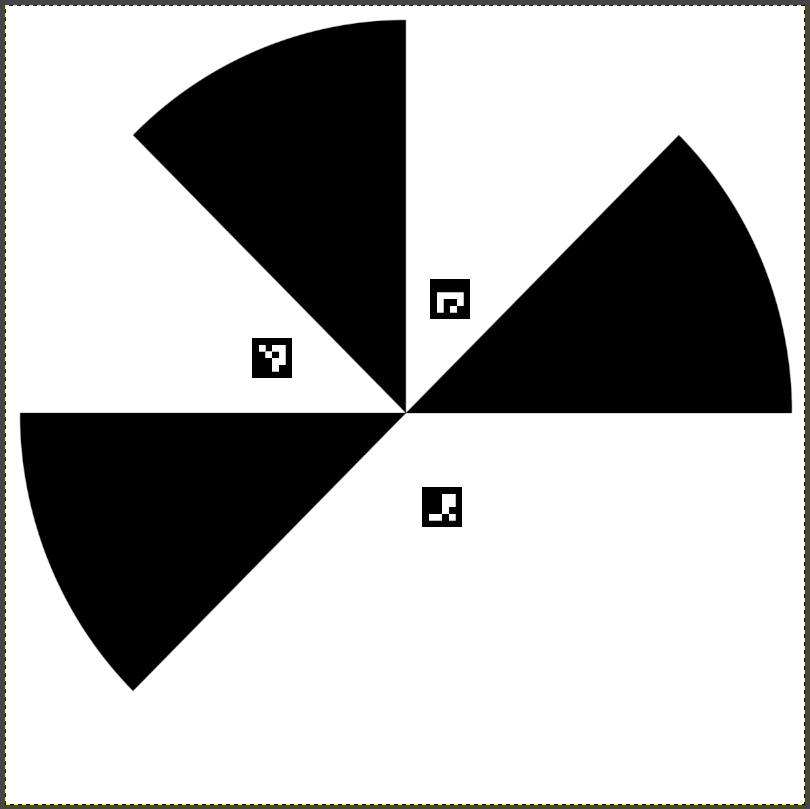
\includegraphics[scale=0.15]{n-fold-for-landing.png}
\caption{The landing marker}
\label{fig:LandingMarker}
\end{figure}

\subsection{Detection of the moving platform}
\label{sec:Detection}

To mark the moving platform a special pattern is constructed,
consisting of an n-fold marker~\cite{NfoldMarker} along with three
ArUco markers~\cite{ArUco_marker} with different ids. This pattern
will be referred to as the \emph{landing marker} and can be seen in
Figure~\ref{fig:LandingMarker}. The n-fold marker is primarily used to
detect the moving platform from a high altitude, while the ArUco
markers are used as extra landmarks in case the marker is partially
visible in the image frame.

% X [Ad3:!] what does it mean different ids?

%[Georgios3:] ids = identifications, like the ID.

To evaluate the computer vision algorithm for detecting the landing
marker, real images of \SI{640}{}$\times$\SI{480}{} pixel size were captured with
an Intel RealSense D435 camera. In the Gazebo simulation a color camera
with the same distortion coefficients as the Intel camera is used to
output a \SI{640}{}$\times$\SI{480}{} pixel image at 10 frames per second (fps).

% X [Ad3:] I'd put the number in the text as it is, but we started with this SI earlier, so now I am just being consistent.

To extract the pixel coordinates of the tip of the n-fold marker, a
kernel size of \SI{13}{}$\times$\SI{13}{} pixels consisting of a real and imaginary
part is created. For every pixel in the image, a convolution is
performed with this kernel and the magnitude of the convolution is
stored. The pixel with the highest magnitude is considered as a
candidate tip of the n-fold marker. For that candidate pixel only, an
estimation of the orientation/phase of the marker is made and an
overall normalized quality score between \SI{0.0}{} and \SI{1.0}{} is calculated. If
the score is above a desired threshold value then the pixel is
accepted as the tip of the n-fold marker. If an n-fold marker is
detected, the result will be the pixel coordinates of the tip of the
n-fold marker along with its orientation/phase.

% X [Ad2:] the sentence "For every pixel in the image, a convolution is performed with this kernel and the magnitude of the convolution is stored." is confusing {maybe me not knowing what a convolution is...}; perhaps "Such kernel is used per each convolution of each pixel in the image while the magnitude of the convolution is being stored." {I actually don't understand at all. 13x13 pixels consist of real and imaginary parts (so I guess is 26x26) which is then iterated; the magnitude is being stored - so 676 per each iteration which is on each pixels but you process 676 pixels at once?}

% [Georgios2:] I think the way I wrote it in the paper is the simplest way to explain it without consuming a lot of space. Otherwise I would have to add equations, figures and then we would need an extra two pages. In computer vision, a convolution is a pixel-wise opearation. For each pixel, a weighted sum of the nearby pixel values is calculated ,according to a kernel size and kernel weights. In our case the kernel size is of 13x13 pixels and the weights are not real numbers but complex numbers (having a real and imaginary part). 

% X [Ad3:] oki doki [but 'the simplest way to explain it' is very definitive. Are you entirely entirely sure of it? ;P]

Since a convolution is a computationally expensive process, an increase
in the kernel size would also increase the computation time and
therefore the energy consumption. However, a higher computation time and energy consumption
is preferred over a non-detection of the n-fold marker. To balance
between energy consumption and effective marker detection, an adaptive
kernel selection function is created to ensure the selection of a
proper kernel size based on a threshold quality score value. In Figure~\ref{fig:NfoldOcclusions} an Intel RealSense D435 Depth camera is used
to capture the image and measure also the distance \emph{d} from the n-fold
marker. Based on a desired quality \emph{q}, the proper kernel size \emph{k} is
selected. It is seen that an occlusion on the tip of the n-fold marker
results in a significant increase in the selected kernel size.

% X [Ad2:] Typo: computationally
% [Georgios2:] Changed "computational" to "computationally".

% X [Ad2:] Typo {the comma typo}: However,
%[Georgios2:] Added the ",".

% X [Ad2:] on the selected -> in the selected
% Georgios2:] Changes that from "on the selected" to "in the selected".

%\hemi{To me this looks like a significant \emph{decrease} in kernel
%  size \ldots}
%
% Georgios: The kernel size, while having an occlusion on the tip of the nfold marker, is 201x201

\begin{figure}[t]
\centering
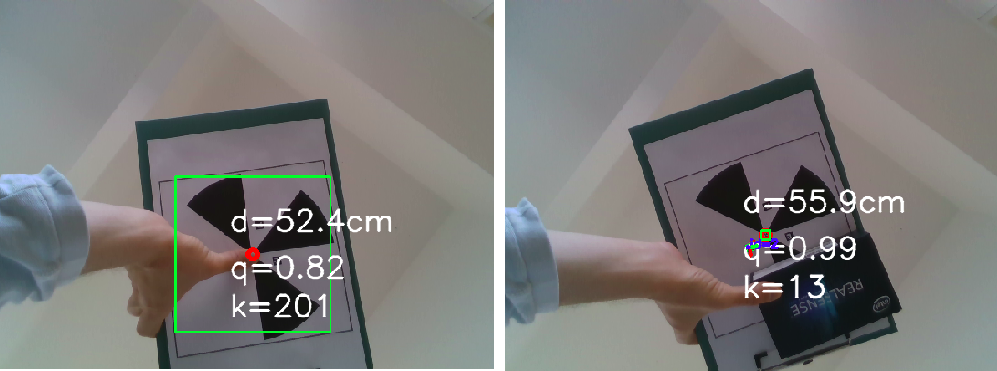
\includegraphics[scale=0.25]{nfold_occlusions.png}
\caption{Detection of the landing marker under different
  occlusions. On the left an occlusion on the tip of the n-fold marker
  and on the right an occlusion on a sector of the n-fold marker.}
\label{fig:NfoldOcclusions}
\end{figure}

%
To detect the ArUco markers the standard OpenCV library is used and if
any ArUco markers are detected, their central pixel coordinates and
pose are stored.

The next step is to convert these pixel coordinates into a real-world
relative position \emph{[X, Y, Z]} according to a local coordinate frame. The
origin of the local coordinate frame \emph{[0, 0, 0]} is defined as the
center of the landing marker and alignment according to the North,
East, Down (\emph{NED}) frame.
% X [Ad3:] here is exactly where putting coordinate frame instead of just frame would just make it
%
%UPS: @Georgios I'm not sure I understand what the NED frame is, can you rephrase or elaborate?
%
The available sensor measurements and sensor fusion algorithms from
the flight controller are used in this process. The PX4 flight
controller outputs through mavlink messages the altitude and the attitude of the UAV (roll, pitch, yaw). For the \emph{Z} component,
the altitude of the UAV from the flight controller's EKF is used. To
obtain the \emph{X, Y} components, an algorithm is constructed to convert
pixel coordinates into real world \emph{X, Y} coordinates in meters:
%
%. This algorithm is described below:
%

% X [Ad2:] it should be NED coordinates? Frame is a navigation frame where we'd have a world one that defines the origin and the body one that define the position of the UAV?
%[Georgios2:] I would stick to NED frame although we could say NED system. For consistency reasons, since we use NED frame everywhere lets stick to it. Concerning world frame and body frame: Both frames are in the 3d world. The body frame has its origin (0,0,0) on the UAV and is aligned to the front side of the UAV. The world frame, in our case the landing site's local coordinate frame has its origin (0,0,0) on the tip of the nfold marker and is aligned to NED frame, meaning it always faces towards the magnetic North.

% X [Ad3:] an open dispute here ;P

% X [Ad2:] will be used sounds like future work. Perhaps is being used?
%[Georgios2:] Agree on that. Changed from "will be used" to "are used"

% X [Ad2:] the altitude of the UAV and the attitude of the UAV (roll,pitch,yaw) -> the altitude and the attitude (roll, pitch, and yaw angles) of the UAV
%[Georgios2:] Agree on that. Changed it accordingly

\begin{enumerate}

\item The pose of the camera in UAV's \emph{BODY} frame is calculated by 
utilizing the roll and pitch IMU data.

% X [Ad2:] a suggestion for next one. Not now as probably we'd have to change a lot: \mathcal{O}_B for body frame, \mathcal{O}_something for some navigation frame; cooler and simpler

\item The normalized coordinates of the four image corners, according to the 
camera's horizontal, vertical field of view and the camera's pose from step 1, 
are calculated.

% X [Ad2:] BODY frame {unless there is a valid reason for BODY pose}
% [Georgios2:] I would stick with pose since the roll and pitch angles of the camera are of interest and therefore included in the pose. Changed from "the camera's BODY pose" to "the camera's pose".

\item The coordinates of the four image corners (in meters), with respect to 
the UAV's \emph{BODY} frame, are determined by using the normalised coordinates from 
step 2 along with the UAV's altitude. The result is a projection plane of the 
image corners on the ground.

% X [Ad2:] The world coordinates -> the coordinates {coordinates in respect of the world reference frame and not world's coordinates}
% [Georgios2:] Rephrased the above paragraph. Hope it makes more sense?

\item The perspective homography matrix is calculated between the two planes, 
the image plane and the world plane from step 3.

% [Ad3:] X two instead of 2 (otherwise I get confused if to use SI)

\item The homography matrix from step 4 is used to convert the pixel coordinates 
of the tip of the n-fold marker from the image plane, into  coordinates (in meters) 
in the UAV's \emph{BODY} frame.

% [Ad2:] X The pixel coordinates are converted into world coordinates -> Pixels are converted into meters {not sure what pixel coordinates are as this is the first time we mention them}
% [Georgios2:] Agree on that. Rephrased it.

\item The coordinates from step 5 are in respect to the UAV's \emph{BODY} frame. 
To convert them into the UAV's \emph{NED} frame, the yaw IMU data from the flight 
controller is used. 

%are converted from the camera's \emph{BODY} frame into the camera's \emph{NED} frame by using the yaw IMU data from the flight controller.

% X [Ad2:] The world coordinates -> the coordinates {coordinates in respect of the world reference frame and not world's coordinates}
% X [Ad2:] are converted from the camera's \emph{BODY} frame into the camera's \emph{NED} frame -> are converted to the \emph{NED} coordinates {NED is not a frame, NED are coordinates or I am totally missing something here}
% {Georgios2:] I rephrased it. Let me know what you think. 

% X [Ad3:] confusing sry ;( I understood you read the position from PX4 in NED coordinate frame. I read UAV frame has it's own coordinate frame which is (0,0,0) that is converted into NED coordinate frame: you just use the reading right? It's not a conversion then

%[Georgios3:] The UAV BODY frame and the UAV NED frame have the same origion but different alignment. The NED always faces the magnetic North while the BODY faces according to the front side of the UAV.

\item The coordinates from step 6, are converted from UAV's \emph{NED} frame 
into the landing site's local coordinate frame.

% X [Ad2:] The world coordinates -> the coordinates {coordinates in respect of the world reference frame and not world's coordinates}
% X [Ad2:] are converted from camera's \emph{NED} frame -> are converted from \emph{NED} coordinates {NED is not a frame, NED are coordinates or I am totally missing something here}

\item For ArUco markers only, an offset vector in the x, y axis is added depending 
on the distance of each ArUco marker from the tip of the n-fold marker. 
It is assumed that this vector is prior known.

\end{enumerate}
%
The mean measurements from the detected n-fold and/or ArUco markers
are used to determine the position and orientation of the landing
marker. The result is an \emph{[X, Y, Z]} relative position of the UAV from
the moving platform along with the yaw orientation of the landing
marker.


\subsection{Navigation}
\label{sec:Navigation}

The purpose of the navigation block is to provide an accurate
prediction for the state of the UAV at any given time. Such a prediction allow us to process images at different fps
according to a desired QoS. Furthermore, the overall robustness of the
system is increased in case the moving platform is not detected in
every image frame. A velocity estimator for the moving platform is
also being implemented as a part of the navigation block.

% X [Ad3:] state -> position; state seems confusing with battery, compoenents
% X [Ad3:] sentence 'This is important because it will allow us to process images at different fps according to a desired QoS.' mmmh; not sure. Not really actually because we don't change QoS dynamically with the position (we actually don't change QoS at all)

% Well ideally we could change it dynamically despite the fact that we are not doing it in this paper.

% [Ad4:] Better not promise what we are not doing (this is new section, so you have the reader reading well here)

The variables of interest that describe the state of the UAV are:
%
\begin{itemize}

\item The relative position of the UAV from the moving platform, 
$x_k\in\mathbb{R}^2$ %\todo[noinline]{I think we might have used a bad name for this value. It currently overlaps with the estimated position of the UAV
%relative to the landing target.}
% [Ad4:] Henrik, that's fine. Clicks, position x, estimated hat_x?
.

% X [Ad3:] confusing; we calculate the position here of the UAV but they are calculated as described in another section. Would erase calculated on, or describe that one is the visual measurement and is used for the purpose of estimation in our EKF.

% [Georgios3:] Agree on that. I deleted it.

\item The attitude of the UAV \emph{[roll, pitch, yaw]}, obtained from the flight controller's IMUs.

\item the velocity of the UAV, $\dot{x}_k$, in \emph{NED} frame, obtained from 
the flight controller's EKF.

% X [Ad2:] NED coordinates
% [Georgios2:]I would stick to NED frame for consistency.

\item the acceleration of the UAV, $\ddot{x}_k$, in \emph{NED} frame, obtained by differentiating the velocities.% X \todo[noinline]{These values are also described on the next page.}

% X [Ad2:] NED coordinates
% [X Ad2:] or ... velocities ->   {How to differentiate velocities? If the velocity is from the flight controller, it's just a value. So we calculate the tangent? I would omit this. Later we don't mention any differentiation but just say they are 'obtained from the flight controller's onboard sensors'}

%[Georgios2:] Considering the calculation of acceleration: Yes we calculate the tangent. We can omit this is you want.

% X [Ad3:] it's little confusing because ... well "which one are you using guys?"; I'd omit still ¯\_(ツ)_/¯ 

%[Georgios3:] Solved. I kept the differentiation of the velocities.

\end{itemize}
%
The altitude, attitude, velocity and acceleration variables of the
UAV's state are obtained from the flight controller's onboard sensors
and already implemented sensor fusion algorithms (EKF). To fuse those
state variables with the obtained position measurements from
Section~\ref{sec:Detection}, a Kalman Filter is implemented. The
measurements from the flight controller are used in the prediction
step.

% X [Ad2:] will be used -> was used {not sure I'd go with future, as normally we use past}
%[Georgios2:] Changed "will be used" into "is implemented"

Prediction Step:\begin{subequations}
\begin{align} 
\hat{x}_{k} & = F \cdot \hat{x}_{k-1} + G_{k} \cdot u_{k}, \\ 
P_{k} & = F \cdot P_{k-1} \cdot F^\top + Q_{k},
\end{align}\end{subequations}
where %$x_k \in \mathbb{R}^2$ is the position of the UAV, 
$u_{k} = \begin{bmatrix}\dot{x}_k & \ddot{x}_k & \dot{x}_{k}^l\end{bmatrix}^\top$ is its control with $x_k,x_k^l$ being the positions of the UAV and the moving platform respectively.
Given $I:=I_2$, a \SI{2}{}$\times$\SI{2}{} identity matrix, the matrix $F=I$, the noise covariance matrix $Q_k=\Delta t_k\cdot\sigma^2_{\textrm{IMU}}\cdot I$, and $\sigma^2_{\textrm{IMU}}\in\mathbb{R}$ is the variance of the velocities retrieved from the flight controller's data. %\todo[noinline]{Is this the right word? 
% [Ad4:] actually no/yes--diatrabes between controls people stating that the model of the system is perfect since is a model [cite Hector]}
Further, \(\Delta t_k\) is the time interval the flight controller output the data (usually around \SI{33}{\ms}). 
The input matrix is given by:
% [Ad4:] Henrik, little lengthy with implicitly saying "is a 2 by 2 identity matrix"
\begin{align*}
G_{k} & = \begin{bmatrix}
    \Delta t_k & 0 & \frac{\Delta t_k^{2}}{2} & 0 & -\Delta t_k & 0\\ 
    0 & \Delta t_k & 0 & \frac{\Delta t_k^{2}}{2} &0 & -\Delta t_k\end{bmatrix},
\end{align*}
% X \todo{
% X  Ad3: Actually $G_k$ might still go easily inline. Something like (commented because latex generates error). Up to you
% X  % Here: $G_k=\Delta t_k\begin{bmatrix}I & \Delta t_kI/2 & -I\end{bmatrix}$
% X }
%The system is initialized with $P_0=I$ and $\hat{x}_0$ coming from the initial measurement.
%where:
% X \todo{
% X  Ad3: the itemize doesn't really add any information the reader doesn't know so far (takes space also)... Makes sense in a thesis, report, not in a paper.
% X }
% \begin{itemize}
% \item  \(x_k \) is the position of the UAV in the landing site's local 
% coordinate system (aligned with NED frame), 
% \item \(\Delta t_k\) is the time interval the PX4's EKF outputs the \(v_x, v_y\) data, 
% usually around 33ms, 
% \item \(\dot{x}_k\) is the linear velocity of the UAV in NED frame, 
% estimated from the PX4's EKF,
% % [Ad2:] NED frame -> NED coordinates
% 
% \item \(\ddot{x}_k\) is the linear acceleration of the UAV in NED frame, 
% estimated on the companion computer from differentiating the velocities.
% 
% % [Ad2:] NED frame -> NED coordinates
% 
% \item \(\dot{x}_k^l\) is the linear 
% velocity of the moving platform in NED frame, estimated from the velocity 
% estimator for the moving platform,
% 
% % [Ad2:] NED frame -> NED coordinates
% 
% \item \(\sigma^{2}_{\textrm{IMU}}\) is the variance of the velocities based 
% estimated by the PX4's EKF.
% % \end{itemize}
% [Ad4:] we are really tight on space and the itemize just rephrase what is said before
% \todo{
%   Ad3: from here to windspeed, I just apply my earlier math suggestion. Henrik, Georgios please check/change/revise.
% }

In the correction step, the observed measurements from the downward
looking camera are used to correct and update the estimated
position of the UAV $\hat{x}_k$. However due to the computation time
needed to detect the landing marker, the incoming measurement is
delayed by a time \(\Delta t_k^{\text{obs}}\in\mathbb{R}_{\geq 0}\). Physically, let us define the displacement $\tilde{x}_k^{\text{obs}}\in\mathbb{R}$ as
\begin{equation}
  \tilde{x}_k^{\text{obs}}:=\bar{\dot{x}}_k\,\Delta t_k^{\text{obs}}, %lol why not->|{\hat{x}_t-\hat{x}_v}|\text{ with }v:=t-d_t^{\text{obs}}, seems you loose the amplitude of the velocity???
\end{equation}
where $\bar{\dot{x}}_k\in\mathbb{R}$ is the mean velocity measured empirically. Such displacement is later employed in the observed measurements. 

Correction Step:
\begin{subequations}
  \begin{align}
    %e_{t} = x^{\text{obs}}_t+\tilde{x}_t - H\cdot\hat{x}_{t} \\<-not necessary
    %S_{t} = H\cdot P_{t}\cdot H^T + R_{t} \\<-easier...
    K_{k} &= P_{k}\cdot H^T(H\cdot P_{k}\cdot H^T + R_{k})^{-1}, \\
    \hat{x}_{k}^f &= \hat{x}_{k} + K_{k}(x^{\text{obs}}_k+\tilde{x}^{\text{obs}}_k - \hat{x}_{k}), \\ %<- TBH not entirely sure why there as there is no system but directly estimate (you would compare the system with the measurement at this step) but ok; if it works then I am fine with it :) [just confirm it does]
    P_{k}^f &= (I - K_{k}\cdot H) P_{k},
  \end{align}
\end{subequations}
where $H=I$, and $x_k^{\text{obs}}$ is the observed position at time $k$. Let us further define $R_k:=\sigma^{2}_{\text{obs}}\cdot I$ where $\sigma^{2}_{\text{obs}}\in\mathbb{R}$ is the variance of the velocities estimated by the PX4's EKF. 

The values of the estimated state $\hat{x}_{k}^f$, and error covariance matrix $P_{k}^f$, are used as input to the next iteration of the prediction step $\hat{x}_{k+1},P_{k+1}$.

A velocity estimator is also constructed to determine the magnitude
and direction of the moving platform's velocity vector. 
The magnitude
is calculated by differentiating two sequential positions 
of the tractor, obtained by detecting the n-fold marker from the 
vertically facing camera as explained in section \ref{sec:Detection}  
and taking into consideration the
UAV's \emph{NED} velocities according to the PX4's EKF. A low-pass
filter is used to provide a smooth estimation of the velocity's
magnitude by filtering out high frequency noise. High frequency noise
can be caused by oscillations of the UAV along with a fast update rate
in the landing marker detection algorithm.  %\hemi{Please explain why
%  the signal is the \emph{smoothest}.}

% [Ad4:] x,y confuses with state

% X \todo{
% X  Ad3: confusing a bit; if we differentiate to estimate the velocity (dx/dt if x is the position) how we use low pass filter to estimate the same velocity we differentiated?
% X }

% [Ad4:] Nobody will notice anyways........ :S

In the agricultural use-case the moving platform is likely to change
its direction up to 180 degrees. Furthermore, it is assumed that the
moving platform is a nonholonomic system, like a tractor. To
compensate for sudden turns, the moving platform's yaw orientation
will be taken into account. Based on the velocity's magnitude and moving platform's yaw orientation, the
moving platform's velocity (\(\dot{x}_k^l\)) in \emph{NED} frame can be obtained.

% [Ad4:] nonholonomic? lol yes and no :P we put just control which is velocity accel velocity of platform and not position (apart init guess); nobody will still notice........ ;S




\subsection{Wind disturbances}
\label{sec:WindDisturbances}
%\todo{
%  Ad3: the force is $F$. Why are we then calling it $force$ later on?
%}
The exact and accurate estimation of the applied wind forces on a body
is a complex matter studied by the field of fluid dynamics. We use a
simplified approach, as follows. We assume that the wind will be
applied on an area of \SI{0.09}{\m^2}. Such an area is emulating a UAV
with extra payload attached on its frame. Two different wind speeds of
\SI{8}{\m \per \s} and \SI{12}{\m \per \s} will be used to calculate the applied wind forces
on that area. The wind forces are considered to be applied on the
center of gravity of the UAV with direction parallel to the ground.

The magnitude of the applied force, corresponding to a certain wind
speed is calculated by the following equations
\cite{Dynamic_pressure_NASA,anderson2010fundamentals}:
\begin{equation}
    \begin{array}{l}
         F_{\textrm{init}} = p_{d} \cdot A,\,\,\,
         p_{d} = \frac{\varrho \cdot v^2}{2},
    \end{array}
\end{equation}%\todo{
%  Ad3: can be one line, and actually, I would trust the reader to search for this one. Is really basic physics.
%}
\noindent where $F_{\text{init}}\in\mathbb{R}$ is the force, \(p_{d}\in\mathbb{R}\) is the dynamic pressure, \(A\in\mathbb{R}\) is
the area of the applied pressure, \(\varrho\in\mathbb{R}\) is the density of the
air (around \SI{1.2}{\kg \per \m^3}), and \(v\in\mathbb{R}\) is the wind velocity in \SI{}{\m \per \s}.

By solving the above equations the applied force on the UAV is found
to be \SI{3.45}{\newton} for an \SI{8}{\m \per \s} wind speed, and 
\SI{7.76}{\newton} for a \SI{12}{\m \per \s}
wind speed. The wind forces are applied on the UAV in Gazebo
simulation, to test the performance of the whole system. This is
done by constructing a program that applies the wind forces on the
virtual UAV.

To simulate a wind pattern the wind direction and magnitude must be
defined. The wind direction is assumed to remain the same for the
whole duration of the experiments. That direction vector is defined as
$w=\begin{bmatrix}0.8 & 0.2\end{bmatrix}^\top$ according to Gazebo's \emph{(x, y)} axes.
%
The magnitude of the wind is calculated as follows: %according to the following pattern:

% [Ad4:] added a name to the direction.

\begin{itemize}
    \item An initial wind force of either \SI{3.45}{\newton} or \SI{7.76}{\newton} is chosen.
    
    \item An update cycle of \SI{5.5}{\second} is chosen between two different applied forces.
    
    \item A random float number between \SI{0.9}{} and \SI{1.2}{} is chosen at every update 
    cycle. This number is defined as $r\in\mathbb{R}$.
    
    \item The applied wind force is calculated as $\hat{F}=w\cdot F\cdot r$ :
%    
%  
%    X \todo{
%    X       Ad3: this is just $F_k=w\cdot F\cdot r$? where $w,r$ is the direction vector you defined earlier \emph{[0.8, 0.2]} and $r$ a random number.
%    X     } 
%        \(\mbox{\em force}_{x} = -x_{norm} * \mbox{\em force} * \mbox{\em Random\_noise} \\
%         \mbox{\em force}_{y} = -y_{norm} * \mbox{\em force} * \mbox{\em Random\_noise}\)\\
%         
%
%    where \(x_{norm } = 0.8\), \(y_{norm}  = 0.2\) 

% [Ad4:] used such direction
\begin{itemize}
    \item For a UAV altitude of \SI{6.0}{\meter} and above, $F=F_{\text{init}}$. % where $F_{\text{init}}$ is either \SI{3.45}{\newton} or \SI{7.76}{\newton}
% [Ad4:] said before.
    \item For a UAV altitude of \SI{6.0}{\meter} and below, the wind force decreases as:
   $F=F_{\text{init}}\cdot h/ 6$ where $h$ is the altitude.
   %, where \(\mbox{\em force}_{init}\) is either \SI{3.45}{\newton} or \SI{7.76}{\newton}
   \item For a UAV altitude of \SI{3}{\meter} and below, $F = 0.5$. 
\end{itemize}
\end{itemize}
%
% [Ad4:] cleaned a little, same meaning.
This model is created to simulate different scaling in the wind's magnitude and is used for all simulated tests.

%%%%%%%%%%%%%%%%%%%%
\section{Evaluation}
\label{sec:experimental}

We evaluate our approach in terms of the quality of the overall
functionality and the energy efficiency of the algorithms. All
algorithms are executed on an embedded companion computer interfaced
to a simulation running on a standard computer.

\subsection{Use-case: agricultural safety}

We evaluate our approach based on a simulated use-case where %We demonstrate the use of 
a multirotor UAV identifies
hazardous objects around a moving platform, and lands on the
moving platform to recharge.
%
%The moving platform is following a path similar to a plowing tractor's and 
%
No communication link is considered between the moving platform and the UAV
and no GNSS positioning is assumed to be available. The system can thus be
considered as a fallback for fault-tolerance.

% [Ad4:] GNSS?

%For the first use, the UAV will track and follow the moving platform from a desired altitude, while detecting and classifying objects on the ground.

Object detection and classification is performed by feeding the input
image from the downward facing camera into a \emph{YOLOv3-tiny} CNN
\cite{yolov3} implemented in ROS \cite{bjelonicYolo2018}. Four
different classes are selected: cars, humans, tractors, and
cows. Based on the CNN's predictions and onboard
sensors, the UAV maps the detected objects onto a 2D map.
 
%For the second use, the UAV will track and land on the moving platform. 

A simulated field is created in Gazebo with objects placed in random
positions and orientations as seen in Figure~\ref{fig:Gazebo}.

\begin{figure}[t]
\centering
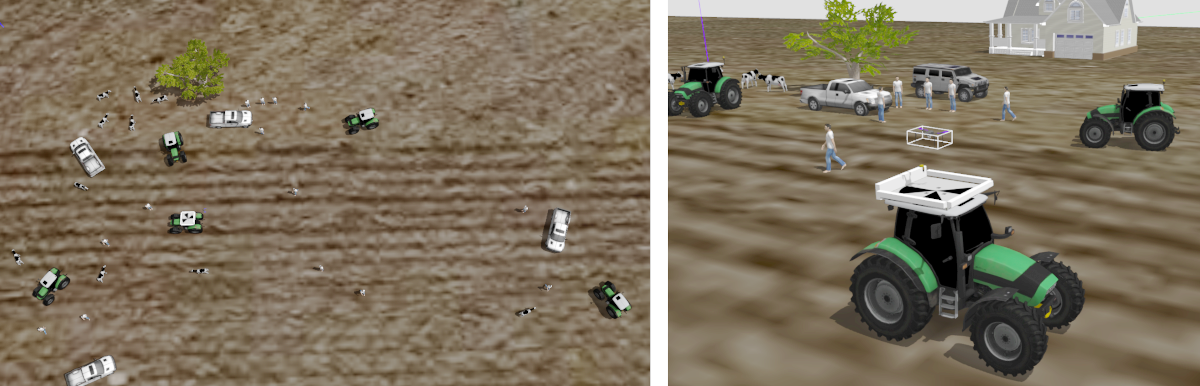
\includegraphics[scale=0.2]{gazebo_scalled_gamma_corrected.png}
\caption{On the left, a top view of the Gazebo scene. 
On the right, a view of the UAV attempting a landing on the moving platform.}
\label{fig:Gazebo}
\end{figure}

Pre-trained weights for \emph{YOLOv3-tiny}, were initially used but the
performance on detecting objects from a downward facing camera was
not satisfactory. Since a dataset for detecting the above four classes
from a top view was not available, we created an artificial dataset
based on the Gazebo models. The dataset consists of 1200 images, 300
for each class. We trained the \emph{YOLOv3-tiny} by its default training
parameters for 5000 epochs, for an input image size of \SI{416}{}$\times$\SI{416}{}
pixels.

%For the following experiments, the input image to $YOLOV3$ $tiny$ will be resized to a 416$\times$416 pixel size. 

\subsection{Experimental setup}

All experiments are performed in Gazebo simulation under Ubuntu 18.04
and ROS Melodic on a i7-8550U 1.8~GHz (4.0~GHz Boost), 8~GB DDR4
laptop. The \emph{PX4} Software In The Loop (SITL) Firmware v1.10.2 is used as the flight
controller and the \emph{IRIS} quadcopter is used as the UAV platform. A
vertically facing RGB camera is placed on the UAV providing a
\SI{640}{}$\times$\SI{480}{} pixel image at 10 fps. An NVIDIA Jetson Nano
with Ubuntu 18.04 and ROS Melodic is used as the UAV's companion
computer. 
%All the computer vision, guidance, and control algorithms 
%execute on the NVIDIA Jetson Nano, similar to how they would
%be deployed if the Nano was a companion computer in a physical drone.
%
% [Ad4:] are we sure KF executes on Nano? Thought it was a pythom sim. Better not stating if not sure
Energy profiling is performed directly on the NVIDIA Jetson
  Nano using \powprof{} as outlined in Section~\ref{sec:semi-automatic}.

Two groups of experiments are conducted. The first group evaluates the
energy consumption and QoS of the \emph{tracking} mode and the second group
evaluates the energy consumption and QoS of the \emph{landing} mode. For
both groups, the experiments start with the tractor moving at a
constant speed of \SI{0.3}{\meter\per\second}, according to a square path similar to that of a
plowing tractor, and the UAV taking off and hovering at an altitude of
\SI{25}{\meter}. After reaching the desired altitude, the UAV starts searching
for the landing marker in the image frame. Once the landing marker is
detected, the UAV commences its actions.

In \emph{tracking} mode, the UAV will follow the moving platform at a fixed
altitude and use its vertically facing camera to map the environment,
while in \emph{landing} mode the UAV will follow the moving platform and
gradually lower its altitude until it lands on it. Both \emph{tracking} and
\emph{landing} modes are tested under three different cases of no wind
disturbances, wind disturbances of \SI{8}{\meter \per \second} and wind disturbances of
\SI{12}{\meter \per \second} according to the wind model described in Section~\ref{sec:WindDisturbances}.


\subsection{Results}

The first group of experiments was conducted to test the \emph{tracking} mode and evaluate its 
energy efficiency and QoS. For the energy 
evaluation, eight tests were executed for different fps rates 
for the \emph{YOLOv3-tiny} ROS node (4fps, 1fps, 0.5fps, 0.1fps) and 
the \emph{landing marker} detection ROS node (10fps, 0.5fps) as 
%
seen in Figure~\ref{fig:PowerDuringTracking}. For a 4fps update rate
for \emph{YOLOv3-tiny}, a power consumption of \SI{6.30}{\watt} is observed while
for a 1fps and 0.1fps update rates, the power consumption drops to
\SI{4,8}{\watt} and \SI{3.9}{\watt} accordingly. By reducing the update rate for
\emph{landing marker} detection, from 10fps to 0.5fps, a further power
saving of \SI{0.15}{\watt}- \SI{0.19}{\watt} is achieved.



For the QoS evaluation, twelve tests were executed for different 
fps rates for the \emph{YOLOv3-tiny} ROS node (4fps, 0.1fps) and for 
the \emph{landing marker} detection ROS node (10fps, 0.5fps) under 
three different cases of wind disturbances. 
%
The QoS is determined as the number of correctly detected objects. An
object is considered to be correctly detected if it is detected within
a distance of \SI{2}{\meter} from the its actual position and classified with
the correct class. The detection results can be seen in
Figure~\ref{fig:NCorrectObjectDetections}. The best results were
obtained for a high fps update rate in \emph{YOLOv3-tiny} and \emph{landing marker} 
detection, under no wind disturbances, since 28 out of the 32
objects were detected. Nevertheless, for the same high fps values but
with a wind speed of \SI{12}{\meter \per \second}, only 18 out of 32 objects were
correctly detected.

%than the fps update rates since for higher wind speed, less objects are correctly detected.





The second group of experiments was conducted to test the \emph{landing} mode
and evaluate its energy efficiency and QoS.
For the energy evaluation, eight tests were executed for different 
fps rates for the \emph{landing marker} detection ROS node 
(10fps, 2fps, 1fps, 0.5fps) using two different cases. 
In the first case, the kernel size remains fixed at 
\SI{22}{}$\times$\SI{22}{} pixels and in the second case an adaptive selection 
kernel size algorithm is used. 
%
The landing time is also taken under consideration as seen in
Figure~\ref{fig:PowerDuringLanding}. The largest difference in the
power consumption is \SI{0.14}{\watt} and is observed between the 0.5fps and
the 10fps update rate for the \emph{landing marker} detection. However
the landing time is reduced by \SI{30}{\second} when using the 10fps update
rate. The adaptive kernel size in most cases outperforms the fixed
kernel size by \SI{0.11}{\watt}. Furthermore the adaptive kernel size can
compensate for marker occlusions which will increase the overall
robustness of the system.

For the QoS evaluation, twelve tests were executed for different 
fps rates for the \emph{landing marker} detection ROS node 
(10fps, 2fps, 1fps, 0.5fps) under three different cases of wind
disturbances. The QoS is determined as the  mean squared error (MSE) 
between the predicted position of the moving platform, 
from the navigation block, and the moving platform's actual position. 
Four different altitude bins were used as seen in 
Figure~\ref{fig:PositionErrorDuringLanding}. 
A large MSE of around \SI{3}{\square\meter} is observed for an altitude 
greater than \SI{20}{\meter} for a 0.5fps rate, while an MSE close to 
zero is observed for an altitude of less than \SI{5}{\meter} for an 
update rate of 10fps. Furthermore, wind disturbances do not seem to 
have an influence on the MSE. We believe the larger MSE for the \emph{y} 
coordinates compared to the \emph{x} coordinates is caused by a 
sudden change of the moving platform's direction on the \emph{y} axis.

\begin{figure}[t]
  \centering
  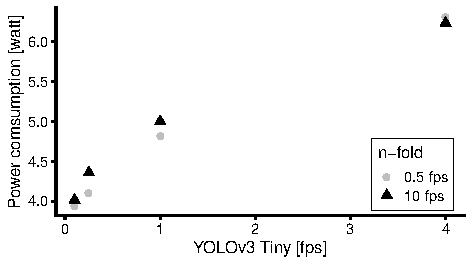
\includegraphics{data_visualization/PowerDetection.pdf}
  \caption{Power consumption during tracking mode. YOLOv3 Tiny fps:
    0=0.1fps, 1=0.5fps, 2=1fps, 3=4fps.}
  \label{fig:PowerDuringTracking}
\end{figure}
  
\begin{figure}[t]
  \centering
  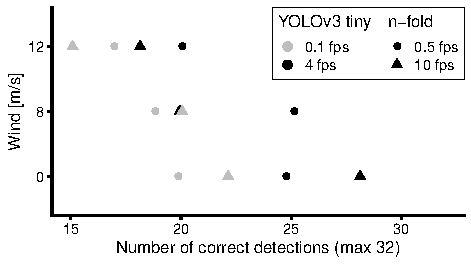
\includegraphics{data_visualization/QoSDetection.pdf}
  \caption{Number of correctly detected objects
  under different conditions. 
  Grey color denotes a 0.1fps and black color denotes a 4fps 
  update rate in \emph{YOLOv3-tiny} ROS node. 
  Circles denote a 0.5fps and triangles denote a 10fps update 
  rate in the \emph{landing marker} detection ROS node.}
  \label{fig:NCorrectObjectDetections}
\end{figure}

\begin{figure}[t]
\centering
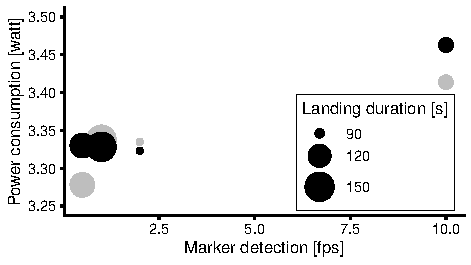
\includegraphics{data_visualization/PowerLanding.pdf}
\caption{Power consumption during landing mode. 
The black circles denote a fixed kernel size while the grey circles denote an adaptive kernel size.}
\label{fig:PowerDuringLanding}
\end{figure}

\begin{figure}[t]
\centering
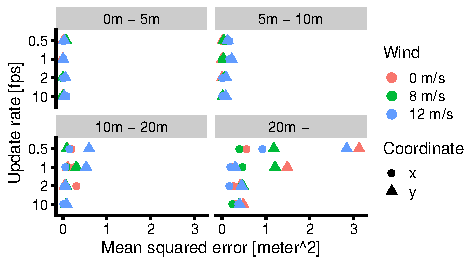
\includegraphics{data_visualization/QoSLanding.pdf}
\caption{Position error during landing and how it depends 
on the marker detection rate at different altitudes and wind disturbances.
Circles denote errors in the x direction and triangles 
errors in the y direction.}
\label{fig:PositionErrorDuringLanding}
\end{figure}

\subsection{Discussion}

The experiments show that both tracking mode and landing mode are
supported by the system, in a simulated environment with a moving
platform and random wind conditions. Moreover, the performance of both
modes is sensitive to the QoS, with a high success rate of both modes
at high QoS levels, and significantly lower performance at lower QoS
levels.

The potential energy savings from having an energy-sensitive algorithm
that can adapt its QoS by changing the fps values for the
\emph{YOLOv3-tiny} and \emph{landing marker} ROS nodes should be seen
in relation to the total energy consumption of the UAV. As a concrete
example, consider a DJI Phantom 4 multirotor and a Sky-Watch Cumulus
fixed-wing (the fixed-wing would need to circle while tracking and 
would need VTOL capabilities to land, but we nevertheless include it 
for comparison). We estimate\footnote{From information on the respective
  product pages regarding battery capacity and maximal flight time.}
that the Phantom uses roughly \SI{140}{\watt} while cruising whereas the Cumulus
uses roughly \SI{40}{\watt} while cruising. The maximal saving gained from
changing the \emph{YOLOv3-tiny} rate is 
$\SI{6.30}{\watt}-\SI{3.9}{\watt}=\SI{2.4}{\watt}$ whereas the
maximal saving gained from changing the \emph{landing marker} rate is
\SI{0.2}{\watt}. For the Cumulus, there is thus a 6.5\% potential energy
saving, whereas the potential energy saving only is 1.9\% for the
Phantom. For the Cumulus this saving is considered large enough to
significantly impact the flying time of the drone, with a total energy
saving of \SI{23.4}{\kilo \joule}. For the Cumulus, the potential saving from adapting
the \emph{landing marker} QoS is however only 0.5\%. 

For the tracking mode, changing the \emph{landing marker} rate
provided a minor saving of \SI{0.14}{\watt}, but at the cost of increased
landing time. Therefore, although the higher-QoS computer vision
algorithm is marginally more expensive by \SI{0.14}{\watt}, the UAV will
overall save energy because of a reduced flight time.

%%%%%%%%%%%%%%%%%%%%%%%%%%%%%%%%%%%%
\section{Conclusion and Future Work}
\label{sec:conclusion}

In this paper we presented a robust, energy-sensitive, vision-based
algorithm for autonomous tracking and landing in varying environmental
conditions, by experimentally executing all the necessary algorithms on 
the NVIDIA Jetson Nano companion computer.
%
% Proposed text by George:
Our experiments show that the proposed computer vision algorithms for 
detecting the moving platform can be run at the highest QoS level with only a marginal
energy overhead, whereas adapting the QoS level of \emph{YOLOv3-tiny} 
CNN results in a considerable power saving for the system as a whole. 
This power saving is significant if the system was executing on a fixed-wing UAV, %
but only marginal if executing on a multirotor UAV.

%Original text by Ulrik:
%Our experience show that the tracking and landing
%algorithms can be run at the highest QoS level with only a marginal
%energy overhead, whereas adapting the QoS level of all on-board
%algorithms results in a significant power saving for the system as a
%whole if it was executing on a fixed-wing drone, but only a marginal
%power saving on a multirotor drone.

In terms of future work, we are interested in automatically adapting
the QoS level to the available battery, and in testing this approach
on a physical drone.

%% acknowledgement
%%%%%%%%%%%%%%%%%%%%%%%%%
\section*{Acknowledgment}

This work is supported and partly funded by the European Union’s
Horizon2020 research and innovation program under grant agreement
No.~779882 (TeamPlay).

\bibliographystyle{IEEEtran}
\bibliography{\jobname} 
\vspace{1ex}

\end{document}
